% !TeX spellcheck = en_US
% This version: Monday August 05, 2024.
\documentclass[12pt, abstracton]{scrartcl}

\usepackage[utf8]{inputenc}
%\usepackage[british]{babel}
\usepackage{lmodern}
\usepackage[table, usenames,dvipsnames]{xcolor}
\usepackage{enumitem}
\usepackage{setspace}
\usepackage{amsmath}
\usepackage{amsfonts}
\usepackage{amssymb}
\usepackage{mathrsfs}
\usepackage{graphicx}
\usepackage[nice]{nicefrac}
\usepackage{xfrac}
\usepackage{marvosym}
\usepackage{lineno}
%\usepackage{doi}
\usepackage{natbib}
\usepackage[titletoc]{appendix}
%\usepackage{ntheorem}
\usepackage{authblk}
%\usepackage{multirow}
\usepackage{booktabs}
\usepackage[labelfont=bf, 
textfont=it,
justification=raggedright,
labelsep=colon]{caption}
\usepackage{tikz}
%\usepackage[nottoc,numbib]{tocbibind}
\usepackage[breaklinks]{hyperref}
\hypersetup{colorlinks, 
	citecolor=blue,
	urlcolor=red}

\renewcommand\Affilfont{\fontsize{9}{10.8}\itshape}

\title{Laboratory Experiments or Opportunistic Abdication: State Governments Behaviour in Times of Pandemic}
\author[$\star$]{Salvatore Barbaro}
\author[$\mp$]{Julia M. Rode}
\author[$ \dag$]{Reyn van Ewijk}
\affil[$\star$,$\dag$]{Johannes-Gutenberg University, Gutenberg School of Management and Economics and Interdisciplinary Public Policy \\ 55122 Mainz, Germany \href{mailto:sbarbaro@uni-mainz.de}{sbarbaro@uni-mainz.de}} 
\affil[$\mp$]{Deutsche Bundesbank, 60431 Frankfurt (HE), Germany}
\date{This draft: \today}

\begin{document}
\maketitle

\begin{abstract}
Federalism may spur beneficial policy experiments that trigger a competition for the best concepts and ideas. For such a competition dynamic to emerge, state governments must have the will and courage to pursue their own paths. Opportunistic behaviors, where state governments shift their responsibilities to the federal level to deflect from their inefficiencies and own failures, pose an obstacle to such policy innovations. The COVID-19 pandemic presented a unique opportunity to scrutinize the behavior of state governments. For Germany, one of the largest federal economies in the world, we collect and analyze data. They show that the behavior of state governments during times of crisis was strongly characterized by opportunistic behavior patterns.
\end{abstract}

\textbf{JEL-Code:} D72, D78,  H77
%%%%%%%%%%%%%%%%%%%%%%%%%%%%%%%%%%
%\newpage 
%\tableofcontents
%\listoffigures
%\listoftables
%%%%%%%%%%%%%%%%%%%%%%%%%%%%%%%%%%%
\linenumbers
\section[Introduction]{Introduction}\label{sec.introduction}
Federal systems can be a boon to society when they induce political innovations through competition, particularly when constituent units (states) act as policy laboratories. The notion of laboratories dates back to Justice Louis D. Brandeis\footnote{
	Justice Louis D. Brandeis in 1932 noted (dissented from the court's opinion) in the New State Ice Co v. Liebmann case (285 US. 262, 311) that "To stay experimentation in things social and economic is a grave responsibility. Denial of the right to experiment may be fraught with serious consequences to the nation. It is one of the happy incidents of the federal system that a single courageous State may, if its citizens choose, serve as a laboratory; and try novel social and economic experiments without risk to the rest of the country."  
} and continues to play a significant role in the collective memory of the United States to this day. The significance of the Brandeis formulation can be gauged by a figure that one might find hard to believe: \cite{Tyler2022} noted that the 'federalism-as-laboratory' statement by Brandeis was referenced over 3,000 times in legal literature alone. Aside from that number, it is widely acknowledged that Justice Brandeis' argument for federalism as a means for policy innovation 'has been accepted by the courts, legal scholars, and policy-makers alike' \citep[p.~49]{InmanRubinfeld2020}.   

A comprehensible reason for this ongoing debate is that its theoretical and empirical core is contentious. Does the conception of political innovations in federalism manifest in practice, or is it merely romanticized like a 'campfire tale' \citep{Tyler2022}?

James \cite{Madison1787} grappled intensely with the question of when a federation can leverage its strengths and what can dim the luster of the federal idea. Madison formulated a condition for the functioning of the federation: Both the central and state layers must embrace the acceptance of divided authority and independent wills with the corresponding power to exercise them. Madison identified opportunistic behavior as a significant impediment to a successful federation. In his \textit{Vices of the Political System of the United States} from 1787, he demonstrated a keen awareness of the dangers posed by strategically driven behavior. 

Indeed, federalist competition can fail if state governments are tempted to exploit the federal union for their own benefit. Because competition is risky for courageous state incumbents, it makes experimentation and self-responsibility perilous for feeble governments. Blurred jurisdiction and shared competencies allow incumbents with poor performance to deflect responsibility. For such strategies, federalism scholars have coined the term transgression \cite[Ch.~3]{Bednar2009} to characterize opportunistic behavior of savvy incumbents. Such transgressions may appear in the shape of encroaching when federal governments usurp states' authority. The states, in turn, may shirk on their obligations to the union. They attempt to position themselves to claim credit for positive outcomes and distance themselves from negative ones. In this context, one strategy is the opportunistic abdication of responsibility  \citep[Ch.~3]{Bednar2009}. It appears when incumbent politicians abandon a policy responsibility. To understand the incentive for abdication, consider that voters do not know the politician type (good vs. bad, well-performer vs. low-performer), a standard assumption in the yardstick competition literature \citep{BesleyCase1995, Revelli2005}. An economic shock (more generally: crisis and disasters) that calls for governmental action will direct attention to incumbent decisions \citep{Graham2023}. The politician knows that her or his behavior will be observed with high awareness by the voters and will eventually affect her or his reelection probability. Bad-performing incumbents can distract from their own responsibility for poor results by claiming responsibility to the central or by hiding behind 'coordinated' decisions.\footnote{
	Evidently, the story can be and has been told in the other direction when federal governments shift responsibility away to the states \citep{Shear2020}. Thus, abdication is a general means to avoid exactly those consequences that yardstick competition promises.}

In this contribution, we present empirical evidence for strategically dominant behavior exhibited by state government leaders during the COVID-19 pandemic. Our empirical analysis focuses on Germany, for which we have collected and evaluated a series of data. We assert with confidence that this work represents the first comprehensive empirical analysis of the strategic behavior of state governments within federal systems. We offer empirical evidence on a theoretically contested subject area.

Indeed, the literature debates whether concerns regarding transgressions are justified. Several authors argued that the incentive for policy innovations are vanished because risk-averse constituent incumbents avoid responsibility for policy failure for which they can make accountable \citep{RoseAckerman1980}. Further, it is not required to assume risk-averse incumbents if voters exhibit a 'negativity bias' \citep{Weaver1986}, i.e., a tendency to be more sensitive to policy failures than to sound decisions. Also, state governments are expected to exhibit a wait-and-see attitude in order to adopt policies only if they have been proved successful in other constituency units. They speculate to free-ride on a horizontal learning externality \citep{Strumpf2002}. On the other side, \cite{KotSchwager2006} underscored the incentive for policy innovation arising from the federal contest, as state politicians can positively influence voters' perceptions of their abilities by successfully implementing policies, especially when they harbor their own political aspirations.

Overall, it must be conceded that research on the innovative capacity vs the opportunistic abdication within federal systems does not yield clear-cut results \citep{Agrawal2022}. Given the political significance of the subject, this is exceptionally regrettable. Ultimately, the unclear state of research is likely attributable to a lack of comprehensive empirical investigation. This deficiency is primarily due to the rarity, if not absence, of the following conditions preferable for empirical assessments of political behavior:

\begin{enumerate}
\item \textbf{Awareness.} There must be a high level of public awareness regarding the policy decisions under consideration. In practice, political decisions, especially at the level of the states, often concern specific groups, yet rarely do decisions attract the interest of the population at large \citep{Boffa2015, Agrawal2022}.
%
\item \textbf{Comparability.} Competition necessitates that voters can compare the decisions of their own government and its outcomes with those of neighboring states. In classical yardstick competition models like  \cite{BesleyCase1995}, a nation-wide shock is assumed that impacts the states uniformly. Often, states face specific issues or concrete challenges that do not arise in comparable forms in neighboring countries. Thus, states are frequently challenged when it comes to decisions following natural disasters such as floods or wildfires. However, these events typically do not occur nationwide. 
\item \textbf{Strategic latitude.} Strategic behavior can only occur when players possess strategic leeway. In federal systems with clear task assignments, decisions cannot be shifted upward or downward. However, when the assignment of a specific task is not clearly attributed to either the states or the federal government (at least in the perception of voters), the possibility for transgressions arises \citep{Hinterleitner2023}.
\end{enumerate}

The COVID-19 pandemic, aside from its devastating impact on humans around the world, has provided a unique opportunity to examine state incumbents' strategic and opportunistic behavior \citep{Kennedy2022}. 

Firstly, the pandemic in general and government decisions to address the challenges drew extraordinary voter interest, making governments highly accountable \citep{Neundorf2021, Algara2022, Singer2022}.

Secondly, the pandemic was a worldwide shock that afflicted the regions in a comparable fashion. Despite the fact that some regions were impacted more than others, e. g.  due to their greater reliance on manufacturing, all states were forced to make decisions regarding, for example, gastronomy restrictions and school closures.

Thirdly, in Germany, where our empirical case is examined, the task of public health protection is primarily a matter for the states, yet the federal government was able to largely assert jurisdiction through concurrent legislation. The states could make significant decisions, such as school closures, entirely autonomously or refer to nationwide agreements.

The last item refers to Germany's tradition of coordinated decision-making \citep{Hegele2017}: the states (Länder) executed the Infection Protection Act but jointly discussed policy measures in (initially) weekly meetings of the Länder with the federal government.  Despite this extensive coordination, a number of Länder made unilateral decisions, while others were oriented towards 'agreed' measures \citep{Hegele2021}. Although 'coordinated decision making' is often positively connoted, ill-performing governments can use it to protect themselves from reputation-damaging comparisons \citep{Keen2013}. In this paper, we investigate whether such opportunistic behavior emerged between the pandemic's onset (spring 2020) and the federal elections in September 2021. In particular, we explore whether low-performing state governments (viz., states with above-average infection rates) promoted unified decision-making while their high-performing counterparts (i.e., those with low infections) preferred state-specific and independent decisions.

To the advantage of the analysis, neither in any state a change in the position of the prime minister took place, nor did the federal government change during the time considered. That allows us to observe each incumbent's behavior over the entire time span. This paper aims to identify confounding factors that will influence the empirical analysis and to establish a positive relationship between the COVID-19 pandemic management performance of a state government represented by the deviation of the seven-day incidence per state from the national average and the call for unified decision-making, that is abdication of federal self-responsibility. 

In a comprehensive empirical framework using official as well as own conducted data, we provide empirical evidence for strategic-driven transgressions. Hence, our results contribute to an ongoing yet inconclusive research on the functioning of federalism as laboratories for policy innovation. 

\section[Federalism in Germany]{Institutional Background: Federalism in Germany}\label{FederalisminGermany}
%
\subsection[The federal structure]{The federal structure}\label{FederalStructure}
Germany's constitution does not prescribe federalism in a refined form, nor does it establish a powerful central government. The term 'unitary federal state' \citep{Hesse1962, Turner2013} aptly characterizes this blended status.\footnote{
	Article 30 of the Basic Law presumes that governmental powers lie with the Länder unless the Basic Law provides otherwise, akin to the Tenth Amendment of the U.S. Constitution. In practice, however, Article 30 was rarely enforced and was labeled a 'living lie' by \cite{Scharpf1994}. Furthermore, Article 70 qualifies Article 30 by stating that the Länder have the right to pass legislation only to the extent that the Basic Law does not grant authority to the central tier.
} The federal polity is often regarded as the archetype of administrative federalism and cooperative decision-making \citep{Kropp2016}. On the federal level, the Länder are represented in the second parliamentary chamber (Bundesrat). They hold a vote on federal laws that trigger the establishment of new administrative proceedings or agencies on the state level \citep{Burkhart2008}, or that impact states' revenues. %Thus, as the number of laws requiring the consent of the Länder increases, the power of their individual parliaments diminishes, while the role of the individual state in federal politics and legislation expands \citep[][p.~394f]{Moore2008}. This results in a highly interconnected political system. %Decisions regarding expenditures and debt are at the discretion of the Länder, but they have almost no tax autonomy. Assuming responsible political action, the German political system frequently necessitates consensus decision-making. \cite{Scharpf1988, Scharpf2006} popularized the term 'joint-decision trap' to describe the tendency of decision-making parties to settle for the lowest common denominator when consensus is regularly sought.  %gekürzt SB 30.07.2024

A particular feature in Germany's constitutional framework is concurrent legislation \citep{Gunlicks2007}, which applies to a variety of policy fields. Among them is the public health responsibility. Concurrent legislation denotes that the Länder have the right to adopt legislation provided the Federation makes no use of its legislative powers in the same field. The Federation has the right to adopt legislation in these fields provided it is intended to establish equitable living conditions in the federal territory or maintain Germany’s legal and economic unity. In this respect, concurrent legislation offers both sides, the states as well as the federal government, opportunities for abdication.

\subsection{Public health responsibilities in Germany's federal polity}
The legal framework governing government intervention during a pandemic is established by the Infection Protection Act (Infektionsschutzgesetz, IfSG). The Länder administer this law, exercising discretion in determining specific measures, their severity, timing, and scope. While the IfSG empowers the federal government to issue recommendations, it also promotes coordination among federal states while allowing flexibility for their actions \citep{Tonti2022}.  

State governments have enacted several measures to curb infections, like the imposition of curfews and limitations on assembly rights and the closing of educational institutions, restaurants, stores, and other facilities. The federal government has retained jurisdiction over border controls. Extensive financial aid packages have been designed by the federal, but were co-financed by the states.\footnote{ 
	The legal framework in Germany also allowed municipalities to chart their own course. Some cities began to take advantage of this opportunity early in the pandemic. The most prominent example is Jena, which was the first city to introduce a requirement for wearing face masks very early on. It became evident that the city of Jena thus generated a prime example of a political laboratory. \cite{Mitze2020} showed that the city’s introduction of masking requirements led to an approximate 25\% reduction in the infection numbers three weeks following introduction. The success in Jena fostered the nationwide compulsory masking.
} 

As already mentioned in the previous subsection, the federal government had the option to take over the tasks handled by the states. However, the federal government did not exercise this authority for the longest time, but only in the summer of 2021 \citep{Rowe2023}, when the pandemic situation had relaxed and most restrictions were lifted.

%As mentioned in the preceding subsection, the federal government possessed the authority to encroach upon state responsibilities via concurrent legislation. However, the federal government refrained from assuming primary responsibility until the summer of 2021, shortly before the majority of restrictions were lifted.


\subsection{Response to the COVID-19 pandemic in Germany's federalism}
Germany was able to weather the COVID-19 pandemic relatively well compared to other industrialized nations. Infection rates, particularly in the autumn of 2020, were relatively low, thus avoiding widespread strain on the healthcare system. 
\begin{figure}[h]
	\centering
	\includegraphics[width = \linewidth]{berfig01.pdf}
	\caption{COVID-19 infections in Germany compared to the other G7 countries and among German states. Source: \cite{Guidotti2022}}
	\label{fig.sevendayincidence}
\end{figure}
The public paid particular attention to infection rates, which were reported by the national health authority in the form of a seven-day incidence rate. This rate is calculated as a moving average over seven days and is expressed in relation to 100,000 inhabitants. The left panel in Fig. \ref{fig.sevendayincidence} depicts this indicator in Germany as well as in the other six G7 countries.

Although infection rates on average were moderate, there were significant differences within Germany (i.e., between the federal states). The right panel in Fig. \ref{fig.sevendayincidence} illustrates the infection rates of the sixteen Länder and marks the nationwide average by the orange-colored line. These values were closely monitored by the public because they were ultimately viewed as the central measure for the possibility of easing the imposed restrictions. Thus, citizens carefully compared how the numbers in their federal state developed compared to other federal states and to the national average \citep{Kaatz2022}.

The national infection control agency, the Robert Koch Institute, which collected and published data on the pandemic, categorizes the infection dynamics into three waves, which are graphically depicted in the right display of Fig. \ref{fig.sevendayincidence}. Wave 1 ran from February 2nd, 2020 till May 17th, 2020; wave 2 from September 28, 2020 till February 28th, 2021, and wave 3 from March 1st, 2021 till June 13th, 2021.

\begin{figure}[h]
	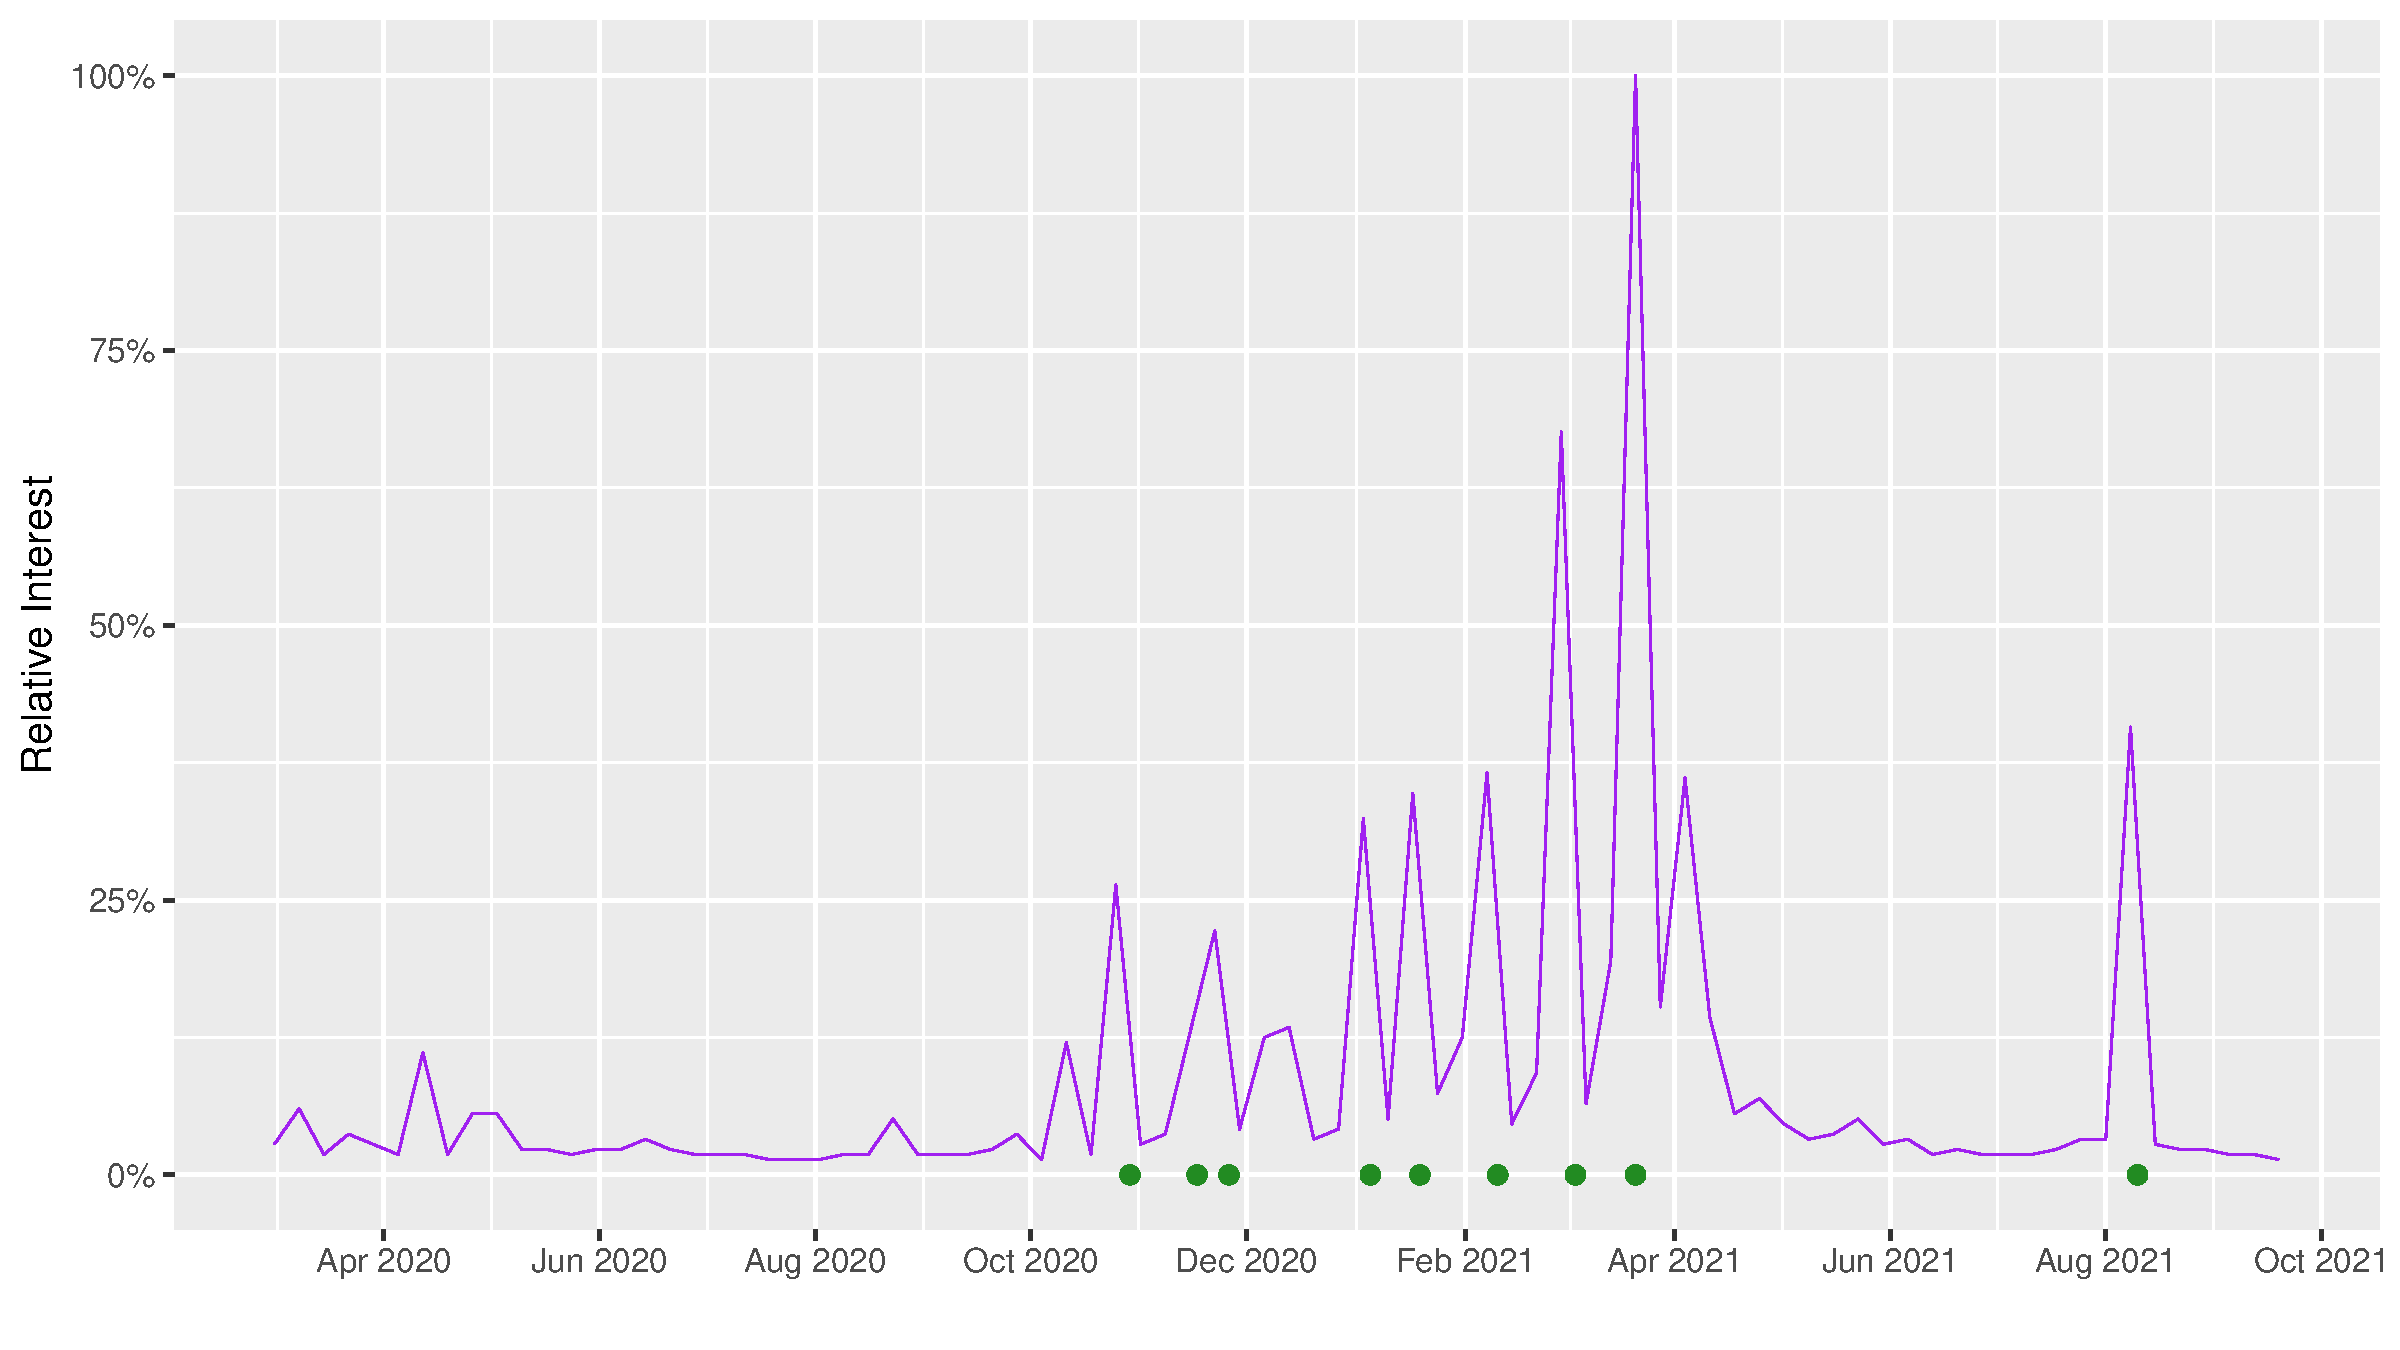
\includegraphics[width=\linewidth]{mpk}
	\caption{Google hits for joint conferences (and related search items).}
	\label{fig.mpk}
\end{figure}

Shortly after the pandemic's onset, state governments were highly interested in policy coordination in joint meetings of states' prime ministers with the chancellor. During the joint meetings, which initially took place quite frequently, the heads of governments agreed on guidelines for crisis management. During the first wave, coordination and uni-directional measures dominated policymaking. While centralized decisions were very rare in the first months after the pandemic's onset, decisions became more heterogeneous (decentralized and unilateral) during the second and third wave \citep{Hegele2021, Kuhlmann2021}.

In the context of this assessment, it is crucial to note the high level of public awareness regarding the outcomes of the joint meetings. To illustrate this awareness, we analyzed data from Google. Figure \ref{fig.mpk} depicts the number of Google searches for the term 'Ministerpräsidentenkonferenz' (the German term for the joint conference) and closely related terms suggested by Google (such as 'results of the joint conference'). The numbers are presented relative to the peak search volume, where a value of 60\% signifies that the searches on a given date amounted to 60\% of the searches on the day with the highest volume. The green dots mark the dates on which the joint conferences occurred. Figure \ref{fig.mpk} indicates that the public showed significant interest in the outcomes of these joint conferences.

Not only did public attention increase rapidly around the time of the meetings, but the statements and opinions of the prime ministers also concentrated heavily on the days immediately following the conferences. We show this analytically in Section \ref{sec.results} (see Table \ref{tb.pmc}). We interpret this as an additional indicator that the conferences received high attention both from political leaders and the public.

%Although the joint conferences still took place roughly every third week, some states decided to act on their own and in contrast to what then-Chancellor Merkel publicly expressed as preferable or even vital. 
From the second wave onwards, the conferences no longer took place weekly as they did after the pandemic's outbreak, but still generally every third week. Despite this high frequency of coordination meetings, some states preferred to take their own measures and deviated from the measures discussed at the conference.

%% To be checked: MPK-Dates and Fig. 2. See: https://de.wikipedia.org/wiki/Bund-L%C3%A4nder-Konferenz


\begin{figure}[h]
	\centering
	\includegraphics[width = \linewidth]{lockdownfig.pdf}
	\caption{Stringency index for relevant restriction measures. Data source: \cite{Steinmetz2022}.}
	\label{fig.lockdown}
\end{figure}

The times and intensity of measures implemented by the Länder to contain the pandemic are summarized in a comprehensive dataset by \cite{Steinmetz2022}. Three particularly salient measures were the stay-at-home requirement ('leavehome'), the closure of schools ('school'), and the closure of childcare facilities ('daycare'). The decisions of the countries to tighten their measures in these areas or to relax the respective restrictions are illustrated in Figure \ref{fig.lockdown}.

Each vertical line denotes a measure adopted by the respective state government, either towards a more stringent regulation (value of 1 or 2) or towards a relaxation (value of 0). Each state is marked by its own color. Figure \ref{fig.lockdown} shows that during the second and especially the third wave, the states did not make their decisions synchronously. In particular, they relaxed measures earlier or later than discussed between the federal government and the states. The data also depicts the homogeneity of policy decisions during the first wave. 

%Yet, research on the political behavior has mainly focused on lawmakers. Utilizing data from parliamentary debates, \cite{Souris2023} revealed instances of blame-shifting and shirking activities among lawmakers. This study suggests that in times of crisis, short-term political success may take precedence over adhering to fundamental convictions. In a related investigation, \cite{Reus2021} assessed the statements of lawmakers in the media during the pandemic. The findings indicated that conservative politicians were more emphatic in defending the federal system than policymakers from other parties. This insight adds a layer to the understanding of lawmakers' responses during a crisis and suggests potential variations in perspectives on federalism among different political groups.
%%% Brauchen wir diesen Abschnitt überhaupt? Ich habe ich jetzt mal rausgenommen, um den gesamten Text etwas zu streamlinen. SB 30.07.2024

%\subsection{Related literature: Political behavior during the COVID-19 pandemic}

\section{Data \& Methods}\label{sec.datamethods}
%\subsection{State governments' positioning during the COVID-19 pandemic}%
%Salva: bitte schaue, ob du meinst, dass wir sub sections brauchen.%
%% Ohne ist besser :) SB 30.07.2024
Our main source of data consists of statements and declarations made by prime ministers of German federal states with respect to COVID-19 management via twitter. We got the data through the twitter API \citep{Kearney2019}. Additionally, we have taken into account press releases and official statements by the respective prime ministers, further enriching our analysis.\footnote{
	The Prime Minister Günther of Schleswig-Holstein gave the last COVID-19 related government declaration by Tweet in January 2021 and replaces them afterwards with oral reports. From Jan. 20th 2021 on, these COVID-19 related oral reports are included instead of Tweets. The Prime Minister Laschet of North Rhine-Westphalia does not give government declarations by tweet during the time of interest. Instead, we utilize COVID-19-related briefings of this state’s government to its local parliament.
	%JULIA: BITTE ÜBERPRÜFE, OB DAS SO STIMMT. DAS HABE ICH AUS DEINER MASTER-ARBEIT SO INTERPRETIERT. (RvE)%
}
%These statements were gathered with a software solution provided by Brandwatch for the time period of interest by defining keywords based upon which the software identifies suitable Twitter statements. %%
%% I replaced this paragr. by a link to the R-package we actually used. SB 30.07.2024

Statements are considered if they indicate preferences/information about the stance of the prime minister regarding central or decentral decision-making. We construct an index measuring state governments’ positioning during the COVID-19 pandemic. This "pandemic policy index" (\textbf{PPI}) measures the extent to which a prime minister, at a given moment during the COVID-19 pandemic, attempts to shift responsibilities to the federal government, the second parliamentary chamber and/or the prime minister conferences. On the one extreme, a prime minister can ask for more regulations at the federal level or criticize that the federal government abdicates, while at the other extreme, a prime minister can state that his/her state will act alone or criticize that the federal government encroaches too much.

Each statement is categorized into four distinct and mutually exclusive categories using an ordinal scale. A value of one indicates that a state prefers to act individually, while a value of four indicates that it asks for more action on the federal level or blames it for problems. Making statements belonging to categories one and two can be interpreted as expressing a preference for federalistic decision-making, and conversely, making statements belonging to categories three and four can be interpreted as expressing a preference for unitary decision-making.

We have summarized our criteria for categorizing all statements in Appendix \ref{app.category}. We also provide in this Appendix two translated examples to illustrate how we applied the categories to the statements.
%We summarized our categorization criteria in Appendix \ref{app.PPI} and  Table~\ref{tb.PPI} presents an overview of the four categories that together constitute the \textbf{PPI}. 
%\begin{table}[h]
	\caption{Categorization criteria federalism index} \label{tbl:PPI}
	\begin{center}
		\renewcommand{\arraystretch}{2}
		\begin{tabular}{  m{1.5cm} | m{3cm} | m{3cm} | m{3cm} | m{3cm} } \toprule 
			value & 1 & 2 & 3 & 4 \\ \midrule 
			& Decide to act individually (state acts on its own) & Support the individual action of the other states & Support deci-sions and actions jointly made with the federal government and/or all other states & Ask for more regulation and action on the federal level \\
			criteria & Criticize that the federal government does too much & Go not along with joint recommendation & Criticize the individual actions of others & Criticize that the federal government does not enough \\
			&  &  & Go along with joint recommen-dation & State holds the federal government accountable for problems \\
			&  &  & Voting for a law but not supporting it &  \\ \bottomrule 
		\end{tabular}
	\end{center}
	\label{tb.PPI}
\end{table}

Categorization criteria were thoroughly predefined in order to ensure a high reliability of the scale. The interrater reliability was tested by letting three independent coders who had been trained in the use of the \textbf{PPI} rate the same statements. %Julia: bitte überprüfe, ob das Vorgehen, das ich hier beschreibe so stimmt.%
The interrater-reliability was calculated using Fleiss’ kappa ($\kappa$) \citep[][Ch.~18]{Fleiss2003},
%Julia: BITTE REFERENZ EINFÜGEN FLEISS (1981): Fleiss, J. L., Levin, B., & Paik, M. C. (1981). The measurement of interrater agreement. Statistical methods for rates and proportions, 2(212-236), 22-23.% Habe die Third Edition von 2003 eingefügt. SB 30.07.2024
which is a generalization of Cohen’s kappa for cases with more than two raters. The kappa statistic compares the observed level of agreement between coders (judges, observers) to the level that is expected under chance. If there is no agreement among coders, then ${\kappa}$ hovers around zero, while ${\kappa}=1$ indicates perfect agreement. Following \cite{Fleiss2003}, a $\kappa$-statistic greater than 0.75 indicates an "excellent" level of agreement. In our case, kappa was 0.91, which implies that rating using the \textbf{PPI} was done reliably and consistently.
% Kappa kann doch sogar negativ sein, oder. Vorher stand da: If there is not agreement among coders, then \kappa >= 0. SB 31.07.2024

Our dataset relies on 600 prime minister statements. Of these, 35.5\%, 6.2\%, 44.8\% and 13.5\% were classified with index values 1, 2, 3 and 4, respectively.

In our study, we investigate whether state governments adapt their stances opportunistically based on their own performance. Specifically, we examine if they favor decentralized decision-making when their performance is good, and shift towards central decision-making when their performance is poor. This analysis is conducted in the context of the COVID-19 pandemic, during which an arguably objective measure of state performance was available. Incidence rates are measured as seven-day moving averages of confirmed cases per 100,000 citizens and are available both at the state level and at the country level \citep{Guidotti2022}.
%Julia: bitte hier eine Referenz zur Datenquelle einfügen. Eine Appendix, die das ganze weiter beschreibt brauchen wir m.E. nicht.%  %% Ich habe Guidotti 2022 als Quelle hinzugefügt, diese haben wir auch benutzt. 
The lower the state-level rate compared to the national average, the better the state's performance. An advantage of this measure is that the data were collected by an authoritative national agency and were widely regarded by the population.

The main ordered logistic regression equation for our analyses is:
\begin{equation} \label{eq.regression01}
 \ln \left( \frac{P(Y \leq j)}{P(Y > j)} \right) = \beta_{j0} + \beta_1 \ln(\text{\texttt{incstate}}_{it}) + \beta_2 \ln(\text{\texttt{incfed}}_{t}) + X' \gamma + u_{it} 
\end{equation}
%Julia/Salva: "=" in meiner Gleichung sieht im Output aus als "-". Kann einer von auch das Problem beheben?% Sollte behoben sein SB 31.07.2024. 
in which $\frac{P(Y \leq j)}{P(Y > j)}$ is the odds of giving a statement falling into category $j$ or lower. $\beta_{j0}$ for $j \in \{1,\ldots,4\}$ give the four category-specific intercepts. \texttt{incstate}$_{it}$ is the incidence rate for state $i$ on date $t$, and \texttt{incfed}$_{t}$ is the federal-level incidence rate on date $t$. In our results, we report the exponent of each coefficient ($\mathrm{e}^{\beta_1}$, etc.) so that the interpretation is in odds. Coefficients larger than 1 imply that an increase in a variable leads to an increase in the odds of giving a statement that lies in a higher category. 

We take the natural logarithm of both \texttt{incstate}$_{it}$ and \texttt{incfed}$_{t}$, so that the coefficient $\mathrm{e}^{\beta_1}$ gives the increase in the odds of giving a higher category statement when the ratio of incidence rate at the state-level divided by incidence rate at the federal level doubles.

An alternative would have been not to include both these variables, but instead measure the deviation between state and federal incidence rate as  $\frac{\text{\texttt{incstate}}_{it} - \text{\texttt{incfed}}_{t}}{\text{\texttt{incfed}}_{t}}$, for which for example a value of zero means that the state rate equals the federal one, and a value of one indicates that the state rate is double that of the federal one. Both specifications only differ in their functional form assumptions. We will show a robustness check in which we demonstrate that the estimated effect sizes in both cases are virtually identical.

In our regression equation, the matrix $X$ includes a set of covariates. These will be included in our regressions in several steps. First, we will control for a linear time trend to capture a potential general trend in stances regarding federalistic decision making. Next, we include a dummy for the five former East German states, and a dummy for the state of Berlin, as there may be differences in policies and attitudes between these states and the western ones. 

Next, we control for the fundamental stances of state governments towards federalism. If a state advocates increased de/centralization, this will not necessarily be driven solely by opportunistic or strategic considerations; ideological convictions can often supersede pragmatic political interests. For example, in the USA, it is known that ideological convictions play a pivotal role in shaping states' and citizens' preferences toward de/centralization. Specifically, conservatives exhibit a genuine attachment to decentralization, while attitudes toward federalism tend to be more instrumental among liberals \citep{Glaser2023, Rendleman2022}. In our context, take, for example, a state government with above-average incidence rates that advocates for decisions regarding school closures or openings to be made collectively and implemented uniformly across the federation. This stance may be opportunistic if the state government generally is in favor of decentral (i.e., federalistic) decision-making, but it may also be congruent with a fundamental belief that the respective state harbors no sympathy for the autonomy of states.

To control for the general stance of the prime ministers, we refer to data from \cite{BarbaroRode2024}, who determined the general stances of state governments based on each state's coalition agreements and prior to the outbreak of the COVID-19 pandemic. The data were classified such that a designation of one signifies a promotion of strong federalism, while four indicates a willingness to cede competencies to the federal level. The resulting average attitude-index values toward federalism for each state are visualized in Appendix \ref{app.stances}, Figure \ref{fig.attitudemap}. 

In the following step, we control for states’ pre-pandemic (2019) share of the manufacturing sector in their gross value added. This variable indicates how strongly each state’s economy was hit by the COVID-19 pandemic \citep{Flach2020}. We furthermore control for states’ financial strength, measured as the sum of states’ tax revenues and the tax revenues of its municipalities, in Germany referred to as states’ financial capacity (“Finanzkraftmesszahl”). In the German redistributive system, financially weak states receive funds out of other states' financial means and additional federal government grants (“financial equalization”). This may affect their stances toward federalistic vs decentral decision-making.\footnote{
	We use 2021 data for this as data for this year most accurately reflect the situation during the pandemic. Moreover, data for pre-pandemic years are less useful as the financial equalization scheme has been reformed. The German statistical office (Statistisches Bundesamt) provides data for this measure.
}  % In den Regressionstabellen ist das durch "State-level controls" berücksichtigt, ja? Da die Finanzkraft aber die generelle Haltung erklärt (Barbaro & Rode 2024), sollten wir diese Variable nicht eher herausnehmen?  

In the final step, we control for the natural logarithm of both the state vaccination rate and the federal vaccination rate at each given date. Data on state- and national-level vaccination rates are available from the epidemiological database for COVID-19 \citep{Guidotti2022}. %Julia: bitte meine Quellenangabe überprüfen und eine Referenz einfügen.% Ich habe unsere Quelle eingefügt (sb, 30.07.2024)

For dates before vaccinations started, both variables receive the value $0$, and a dummy variable for the pre-vaccination period is included. State vaccination rates, relative to federal vaccination rates, can be thought of as another measure of the success of local policies, although they less clearly result from policies and interventions at the state level than is the case for incidence rates.\footnote{
	The federal government was responsible for procuring the vaccine doses, but the states were in charge of organizing the vaccinations. Each state had its own vaccination centers and its own procedures for scheduling vaccination appointments. For example, some states offered vaccinations in buses that traveled to university campuses and smaller towns. Therefore, high vaccination rates can indeed be attributed to the high administrative quality of the respective states.
} Moreover, access to vaccinations was only possible starting in January 2021.  % Footnote added to strenghten the usage of the vacc. variable. SB 31.07.2024

In our analyses, we utilize prime minister statements from waves 2 and 3 of the pandemic. Before wave 2 started, incidence rates were considerably less reliably recorded. Measurement error in the initial phase of the pandemic may have differed between states, and potentially so in an endogenous way. Moreover, during wave 1, and especially the period between waves 1 and 2, the difference between state-level and federal-level incidence rates measured in percentages fluctuated wildly as reported rates were often low.

In our ordered logistic regression, the coefficients $\beta_1$, $\beta_2$ and $\gamma$ are assumed to be the same across all categories. We test this proportional odds assumption for our main model using a likelihood ratio test \citep{Brant1990} and find no evidence for a violation of this assumption: the null hypothesis of equality of the coefficients is not rejected with $\chi^2 (22) = 29.25$, $p = 0.14$. $u_{it}$ is an error term. Standard errors are clustered at the date level to account for any between-state correlations that arise because during the pandemic all states often experienced similar events (e.g., pandemic-related news) at the same moment.  % I added the Brant 1990-reference. OK? SB 31.07.2024

%In a robustness check, we exclude the states of North Rhine-Westphalia and Bavaria from the data, because …………………… %Julia/Salva: bitte ergänzen.%
%% neu eingefügt (SB 31.07.2024): 
During our study period, the prime ministers of North Rhine-Westphalia and Bavaria fiercely and publicly contested the chancellor candidacy of the conservative parties (CDU and CSU). Both tried to distinguish themselves with their own positions on handling the pandemic \citep{Jun2023}. Therefore, it is possible that the internal party campaign biased the statements of these two prime ministers. We excluded these two states in a robustness check to account for this.
%% (SB 31.07.2024)

In a further robustness check, we conduct a state fixed effects (conditional) ordered logistic regression. This has the advantage of relying solely on within-state variation but has two drawbacks. First, we lose a lot of the variation of interest and, therefore, statistical power. Second, this method cannot be estimated when the clustering of the standard errors is at a different level (here: date) than the grouping variable (here: state). Hence, some relevant autocorrelation is ignored, while clustering occurs for a low number of groups (16 states), which might lead to inconsistent standard errors.

During the pandemic, the joint conferences of the state prime ministers were closely watched by the population as many of the central pandemic-related interventions were discussed and decided upon. We expect that prime ministers will have been especially likely to make their stance with respect to central or decentralized decision-making clear in the week around these conferences and perhaps most so in the days immediately following such a conference. We, therefore, conduct two sets of analyses. First, we analyze to what extent the number of statements issued per day changed during the week of a conference (three days before, till three days after the conference), and immediately after a conference (day of the conference till three days afterwards). For this, we calculate the number of statements issued per day and regress this on a linear time trend and a dummy indicating the time period right around / right after the prime minister's conference. Second, we conduct our main analyses using the specification that includes all controls while limiting the data to the time period right around / right after prime ministers' conferences.

\section{Results}\label{sec.results}
\subsection{Main Analysis}
%Salva/Julia:
%I uploaded the tables in pdf and Excel format. These could be made nicer-looking by turning them into Latex-code.
%I here give a brief overview of results. It would be great if you could provide the story around this. I can later of course also still write on this section and describe the estimates from the methods viewpoint so that it aligns with the Data & Methods section.
%%%% TABLE 1 (SB) - 30.07.2024
The results of the regression analysis for Equation (\ref{eq.regression01}) are shown in Table \ref{tb.reg01}, with the last three rows representing the covariates. The dependent variable is a 4-point ordinal scale with higher scores indicating a stronger preference for unitary (centralized) decision-making.

\begin{table}[htbp] 
	\centering
\caption{Covid-19 incidence rates and state prime ministers' statements favoring (de)centralized decision-making}
 \label{tb.mainreg}
\begin{tabular}{lccccc} \toprule
    & (1) & (2) & (3) & (4) & (5) \\ \midrule
ln(state-level  & 1.730** & 1.904*** & 2.003*** & 1.983** & 1.985** \\
\, incidence rate)	& [1.22,2.45] & [1.34,2.70]  & [1.41,2.85]  & [1.30,3.02]  & [1.29,3.06] \\
 & & & & & \\
ln(state-level  &  &  &  &  & 0.806 \\
\, vacc. rate)		&  &  &  &  & [0.606,1.072] \\
		& & & & & \\
Linear time trend & No & Yes & Yes & Yes & Yes \\
		& & & & & \\
Dummies Eastern  &    &    &     &     & \\
\,  states and Berlin  & No & No & Yes & Yes & Yes \\ 
		& & & & & \\
State-level controls & No & No & No & Yes & Yes \\ \\ \midrule
 Observations & 600 & 600 & 600 & 600 & 600 \\		\bottomrule
\end{tabular}
\label{tb.reg01}
\begin{minipage}{\textwidth}
	\small
\textit{Notes:} Each column reports exponentiated coefficients from a separate ordered logit regression. Dependent variable is the 4-point pandemic policy index (PPI). Higher values indicate a stronger expressed desire for centralized decision-making. Coefficients are expressed as changes in the odds ratio of giving a statement $Y$ that falls into a higher vs a lower category $j$, i.e., $P(Y\leq j)/P(Y > j)$. All regressions control for ln(federal level incidence rate) and column (5) additionally controls for ln(federal level vaccination rate) and a dummy for the pre-vaccination period. State-level controls include states' general stances towards federalism, share of the manufacturing sector in gross value added, and financial strength ("Finanzkraftmesszahl"). \newline \textit{*** $p < 0.01$, ** $p < 0.05$, * $p < 0.10$}
	\end{minipage}
\end{table}

The table presents exponentiated coefficients from an ordered logistic regression. The coefficient to the natural log of state-level incidence rates gives the increase in odds $\left( \frac{P(Y \leq j)}{P(Y > j)} \right)$ of giving a statement that falls into category $j$ or lower. Coefficients larger than one indicate that an increase in an independent variable leads to higher scores on the \textbf{PPI}, while coefficients smaller than one indicate the opposite. Increases in incidence rates in a state relative to the country-wide level lead prime ministers to display a greater preference for centralized decision-making. If the incidence rate in a state doubles compared to that at the federal level, the odds of giving a statement that is categorized as being one point higher on the \textbf{PPI} also roughly doubles.

As can be seen by comparing columns (1) to (5), the main result is robust throughout all specifications.  The coefficient to the log of the state-level vaccination rate suggests that higher vaccination rates in a state, compared to the nationwide average, lead prime ministers to give more federalistic statements, i.e., more strongly in favor of decentralized decision-making.


%Table 1:
%\begin{itemize}
%%\item The dependent variable is  4-point ordinal scale with higher scores indicating a stronger preference for unitary (centralized) decision-making.
%%\item The table presents exponentiated coefficients from an ordered logistic regression. The coefficient to the natural log of state-level incidence rates give the increase in odds ($\frac{P(Y \leq j)}{P(Y > j)}$) of giving a statement that falls into category $j$ or lower. Coefficients larger than 1 indicate that an increase in an independent variable leads to higher scores on the \textbf{PPI}, while coefficients smaller than 1 indicate the opposite.
%%\item Increases in incidence rates in a state relative to the country-wide level, lead prime ministers to display a greater preference for centralized decision-making.
%%\item If the incidence rate in a state doubles compared to that at the federal level, the odds of giving a statement that is categorized as being one point higher on the \textbf{PPI} also roughly doubles.
%%\item This result is robust throughout all specifications (compare columns 1-5).
%%\item The coefficient to the log of the state-level vaccination rate suggests that higher vaccination rates in a state, compared to those at the federal level, lead prime ministers to give statements that are more federalistic in nature, i.e., more strongly in favor of decentralized decision-making.
%\end{itemize}

\subsection{Robustness Checks}
As outlined in the previous section, we conducted a series of robustness checks. The first concerns the two prime ministers who were in an intra-party competition during the observation period. In fact, these two prime ministers made the most statements. Therefore, the intra-party campaign could distort the results. As part of our first robustness check, we repeated the regression analysis, but without the data from these two states.

\begin{table}[htbp]
%	\centering
\caption{Robustness checks: COVID-19 incidence rates and state prime ministers' statements favoring (de)centralized decision-making}
\begin{tabular}{lcccc}		\toprule
  & Excluding NW & Deviations in- & Fixed & Fixed \\
  & and BY       & stead of logs & effects & effects \\
  & (1) & (2) & (3) & (4) \\	\midrule
ln(state-level  & 2.145*** &  & 1.610 & 1.504  \\
\, incidence rate)  & [1.38,3.33] &  & [0.91,2.86] & [0.86,2.63]   \\
  & & & & 			\\
ln(state-level   & 0.751* &  & & 0.740**   \\
\, vacc. rate)  &   [0.58,0.97] & & & [0.56,0.98]   \\
  & & & &		\\
Perc. diff.: state- vs   &  & 1.956** &  &  \\
\, fed.-level incid. rate &  & [1.17,3.25] &  &  \\
  & & & &			\\
Perc. diff.: state- vs       &  & 0.961 &  &  \\
\, fed.-level vacc. rate	&  & [0.10,9.22]  &  &  \\
 & & & &		\\
Linear time trend & Yes & Yes & Yes & Yes \\
& & & & \\
Dummies for Eastern  & Yes & Yes & No & No \\
\, states and Berlin & & & & \\
 & & & & \\
State-level controls & Yes & Yes & No & No \\
 & & & & \\
State fixed effects & No & No & Yes & Yes \\
 & & & &		\\ \midrule
 Observations & 479 & 600 & 600 & 600 \\		\bottomrule
\end{tabular}		
\label{tb.reg02}
\begin{minipage}{\textwidth}
\small 	\textit{Notes:} Columns (1), (3) and (4) each report exponentiated coefficients from a separate ordered logit regression. In columns (3) and (4), these are state fixed effects (conditional) ordered logistic regressions. Dependent variable is the 4-point pandemic policy index (PPI). Higher values indicate a stronger expressed desire for centralized decision-making. Coefficients are expressed as changes in the odds ratio of giving a statement $Y$ that falls into a higher vs a lower category $j$, i.e., $P(Y \leq j)/P(Y > j)$. Column (2) shows results from a regression in which the independent variable of interest is measured as percent difference between state-level and federal-level rates. Regressions (1), (3) and (4) control for ln(federal level incidence rate). Regressions (1) and (4) additionally control for ln(federal level vaccination rate). Regressions (1), (2) and (4) include a dummy for the pre-vaccination period. State-level controls include states' general stances towards federalism, share of the manufacturing sector in gross value added, and financial strength ("Finanzkraftmesszahl").
\newline \textit{*** $p < 0.01$, ** $p < 0.05$, * $p < 0.10$}
\end{minipage}
\end{table}

Table \ref{tb.reg02} presents the regression results. From the comparison of Tables \ref{tb.reg01} and \ref{tb.reg02} it becomes evident that the two coefficients for the incidence rates of the respective states differ only slightly from each other (1.73 vs 1.75). However, the significance level decreases somewhat due to the exclusion of the two states but remains at a high level.

In the next robustness check, we do not include the logs of the state- and federal-level rates, but instead take the relative difference between both rates, with e.g., a value of one indicating that the state rate is double that of the federal one. The estimates are almost the same as in the main analyses.  %% I struggle with the table here. If the original variable is omitted and replaced with the 'relative difference'-variable, why is there still a number for the original variable in col (2)? SB 30.07.2024

Finally, in columns (3) and (4), we show the results from fixed effects (conditional) ordered logistic regressions. The results should be treated with some caution because of the drawbacks (different levels of standard-error clustering) on which we pointed to at the end of Section \ref{sec.datamethods}. The point estimates are robust to the inclusion of fixed effects, though coefficients are slightly smaller than in our main analyses.

Regarding the influence of vaccination rates, the robustness checks show a similar coefficient to the main analysis. However, the vaccination rate becomes significant at the 95\% level when the states of Bavaria and North Rhine-Westphalia are excluded as well as in the fixed-effect specification. The coefficients are smaller than one, which indicates that if state-level vaccination rates increase relatively to the federal-level, prime ministers tend to propagate more decentralized decision-making.

The significant effect of the vaccination rate may be seen as a further indicator of our main hypothesis, according to which above-average success (in this case: higher vaccination rates than the national average) motivates the state prime ministers to emphasize the states' own responsibility and self-determination more strongly. 	

Nevertheless, we would not overestimate the regression results regarding the vaccination rate and would interpret the results with caution. Firstly, because the coefficient to this particular variable in our main analysis in Table \ref{tb.reg01} is not significant. Secondly, the above-reported fact that vaccination doses were only feasible starting in January 2021 limits the statistical power to find effects.


%\newpage
%Table 2 – robustness checks:
%\begin{itemize}
%\item The results are robust to the exclusion of the states of North Rhine-Westphalia and Bavaria from the data. (I was not sure why we did this. Please briefly mention here. A slightly longer description should go into the Data \& Methods section.)
%\item In the next robustness check, we do not include the logs of the state- and federal-level rates, but instead take the relative difference between both rates, with e.g., a value of 1 indicating that the state rate is double that of the federal one. The estimates are almost the same as in the main analyses.
%\item Finally, in columns (3) and (4), we show the results from fixed effects (conditional) ordered logistic regressions. The results should be treated with some caution because (see Data section). The point estimates are robust to the inclusion of fixed effects, though coefficients are slightly smaller than in our main analyses.
%\item Note that in the analysis that excludes North Rhine-Westphalia and Bavaria, as well as in the fixed effects analysis in column (4), the effect of vaccination rates becomes significant. The coefficients are smaller than 1, which indicates that if state-level vaccination rates increase relatively to the federal-level, prime ministers tend to propagate more decentralized decision-making.
%\item \textit{I think we can add the results for vaccination rates as additional evidence for our hypothesis that more success at the state-level leads local politicians to call for more decentralized decision-making. However, we do have to be a bit careful with this. First, because the coefficient to the vaccination rate variable in our main analysis in Table 1 is not significant. And second, because of what I wrote in the Data \& Methods section:
%“State vaccination rates, relative to federal vaccination rates, can be thought of as another measure of the success of local policies, although they less clearly result from policies and interventions at the state-level than is the case for incidence rates. Moreover, vaccinations only became available in January 2021.” (The latter sentence implies that the statistical power to find effects is smaller.)}
%\end{itemize}

\subsection{Focusing on the time around the conferences}
The previous analyses include all data points during the second and third waves, partially excluding two states. We argued that public awareness was particularly high on the days around the conferences of the heads of government (see Fig. \ref{fig.mpk}). This means, conversely, that statements by the prime ministers on days with lower attention are weighted the same as statements on days with very high attention to the topic of COVID-19. Prima facie, it cannot be ruled out that the results are biased by statements that were less intensely perceived, which could lead to misinterpretations of our findings.

\begin{table}[htbp]
%	\centering
\caption{Numbers of statements per day around prime ministers conferences (PMC)}
\begin{tabular}{lccc}	\toprule
    & (1) & (2) & (3) \\	\midrule
Week of PMC & 1.786*** &  &  \\
    & (0.492) &  &  \\
    & & &			\\
3 days before PMC &  & 0.081 &  \\
    &  & (0.422) &  \\
    & & &			\\
Day of PMC till 3 days afterwards &  &  & 2.672*** \\
    &  &  & (0.727) \\
    & & &			\\ \midrule 
Observations & 289 & 289 & 289 \\ \bottomrule
\end{tabular}
\label{tb.pmc}
\begin{minipage}{\textwidth}
\small
\textit{Notes:} Each column reports results from an OLS regression in which each observation contains the number of statements (tweets) given by state prime ministers per day. Each regression corrects for day of the week fixed effects and includes a dummy indicating a period around the PMCs. In column (1), this is the time period from three days before till three days after PMCs, in column (2), this is three days before PMCs and in column (3), this is the days of PMCs $+$ 3 days afterwards. \newline \textit{*** $p < 0.01$, ** $p < 0.05$, * $p < 0.10$}.
	\end{minipage}
\end{table}

In order to address this, we firstly examine whether the prime ministers made their statements particularly in the context of the conferences. Then, we re-run our above analysis using only the statements made around the time of the conferences.

First, the statements of the prime ministers do indeed concentrate around the conferences. Table \ref{tb.pmc} depicts this.
	
In the week around prime minister conferences (3 days before till 3 days after), prime ministers issue more statements: around 1.8 more statements (tweets) are issued per day. This effect is entirely concentrated in the time immediately after the PMCs: the number of tweets (statements) per day does not increase in the 3 days prior to a PMC, but in the period between the PMC and 3 days afterwards, around 2.7 more statements are issued by prime ministers daily.

\begin{table}[htbp]
%	\centering
\caption{Covid-19 incidence rates and state prime ministers' statements favoring (de)centralized decision-making around the prime ministers conferences}
\begin{tabular}{lcc} \toprule
    & Week of prime ministers & Day of PMC till \\
    & conference (PMC)        & 3 days afterwards \\
    & (1) & (2) \\ 		\midrule
ln(state-level incidence rate) & 2.436** & 3.482** \\
    & [1.26,4.71] & [1.62,7.47]  \\
    & & \\
ln(state-level vaccination rate) & 2.526 & 0.467 \\
    & [0.07,91.21] & [0.01,22.14]  \\
    & & \\
Linear time trend & Yes & Yes \\
Dummies for Eastern & Yes & Yes \\
\, states and Berlin & & \\
State-level controls & Yes & Yes \\
& & \\ \midrule
Observations & 294 & 223 \\ \bottomrule
\end{tabular}
\label{tb.regpmc}
\begin{minipage}{\textwidth}
\small
\textit{Notes:} Each column reports exponentiated coefficients from a separate ordered logit regression. Column (1) limits the sample to the week around prime ministers conferences (PMC). Column (2) limits the sample to the days of PMCs $+ 3$ days afterwards. Dependent variable is the 4-point pandemic policy index (PPI). Higher values indicate a stronger expressed desire for centralized decision-making. Coefficients are expressed as changes in the odds ratio of giving a statement Y that falls into a higher vs a lower category j, i.e., $P(Y\leq j)/P(Y>j)$. Both regressions control for ln(federal level incidence rate), ln(federal level vaccination rate) and a dummy for the pre-vaccination period. State-level controls include states' general stances towards federalism, share of the manufacturing sector in gross value added, and financial strength ("Finanzkraftmesszahl"). \newline \textit{*** $p < 0.01$, ** $p < 0.05$, * $p < 0.10$}
	\end{minipage}
\end{table}

Secondly, we re-run the main analysis but now focus on the week of PMCs (Table \ref{tb.regpmc}, column (1)) and the period between a PMC and 3 days afterward (column (2)). It turns out that directly following a PMC, prime ministers respond especially strongly to the perceived successfulness of their policies as measured by state-level incidence rates. The odds ratio increases to 3.5. This implies that a doubling of the incidence rate in a state compared to that at the federal level leads to 3.5 times higher odds of giving a statement that falls into a higher category of the \textbf{PPI}. Thus, if we focus on those statements that received particular attention, then the effect we examined is even stronger than in the main analysis. We interpret this as a reinforcement of our core finding.

\section{Conclusion}

\newpage

\bibliographystyle{elsarticle-harv}
\bibliography{ber}

\newpage
\appendix
\renewcommand{\thefigure}{A\arabic{figure}}
\counterwithin{figure}{section}

\section{Categorization Criteria for the Federalism Index}\label{app.category}
\begin{table}[h]
	\caption{Categorization criteria federalism index} \label{tbl:PPI}
	\begin{center}
		\renewcommand{\arraystretch}{2}
		\begin{tabular}{  m{1.5cm} | m{3cm} | m{3cm} | m{3cm} | m{3cm} } \toprule 
			value & 1 & 2 & 3 & 4 \\ \midrule 
			& Decide to act individually (state acts on its own) & Support the individual action of the other states & Support deci-sions and actions jointly made with the federal government and/or all other states & Ask for more regulation and action on the federal level \\
			criteria & Criticize that the federal government does too much & Go not along with joint recommendation & Criticize the individual actions of others & Criticize that the federal government does not enough \\
			&  &  & Go along with joint recommen-dation & State holds the federal government accountable for problems \\
			&  &  & Voting for a law but not supporting it &  \\ \bottomrule 
		\end{tabular}
	\end{center}
	\label{tb.PPI}
\end{table}

In the following, we provide two translated examples to illustrate the categories: 

\begin{quotation}
	%I believe it is unhelpful to pit the states against the federal government. It can only work if we work together. The federal legislators have the opportunity to integrate everything into the Infection Protection Act and to debate everything that we are debating. 
	But I want to make it very clear: I believe the past few days have shown that it is important for us in Mecklenburg-Western Pomerania to follow our own path.
\end{quotation}
%Source: Manuela Schwesig, Mecklenburg-Vorpommern, "Plenarprotokoll_7_117" p. 7%

This statement by Prime Minister Manuela Schwesig of Mecklenburg-Western Pomerania is classified into category one. In contrast, the following statement by Prime Minister Stephan Weil of Lower Saxony is classified into category four.
\begin{quotation}
	My claim towards the federal government is: rapid approval of the tests and an ambitious, preferably nationwide test strategy.	
\end{quotation}
%Source: Stephan Weil, Niedersachsen,"Fortschritte, Risiken und Perspektiven – Niedersachsen kämpft mit dem Corona-Virus Regierungserklärung des Niedersächsischen Ministerpräsidenten Stephan Weil vor dem Niedersächsischen Landtag am 17. Februar 2021", p. 12%


\newpage
\section{States' attitudes toward federalism}\label{app.stances}
\begin{figure}[h]
	\centering
	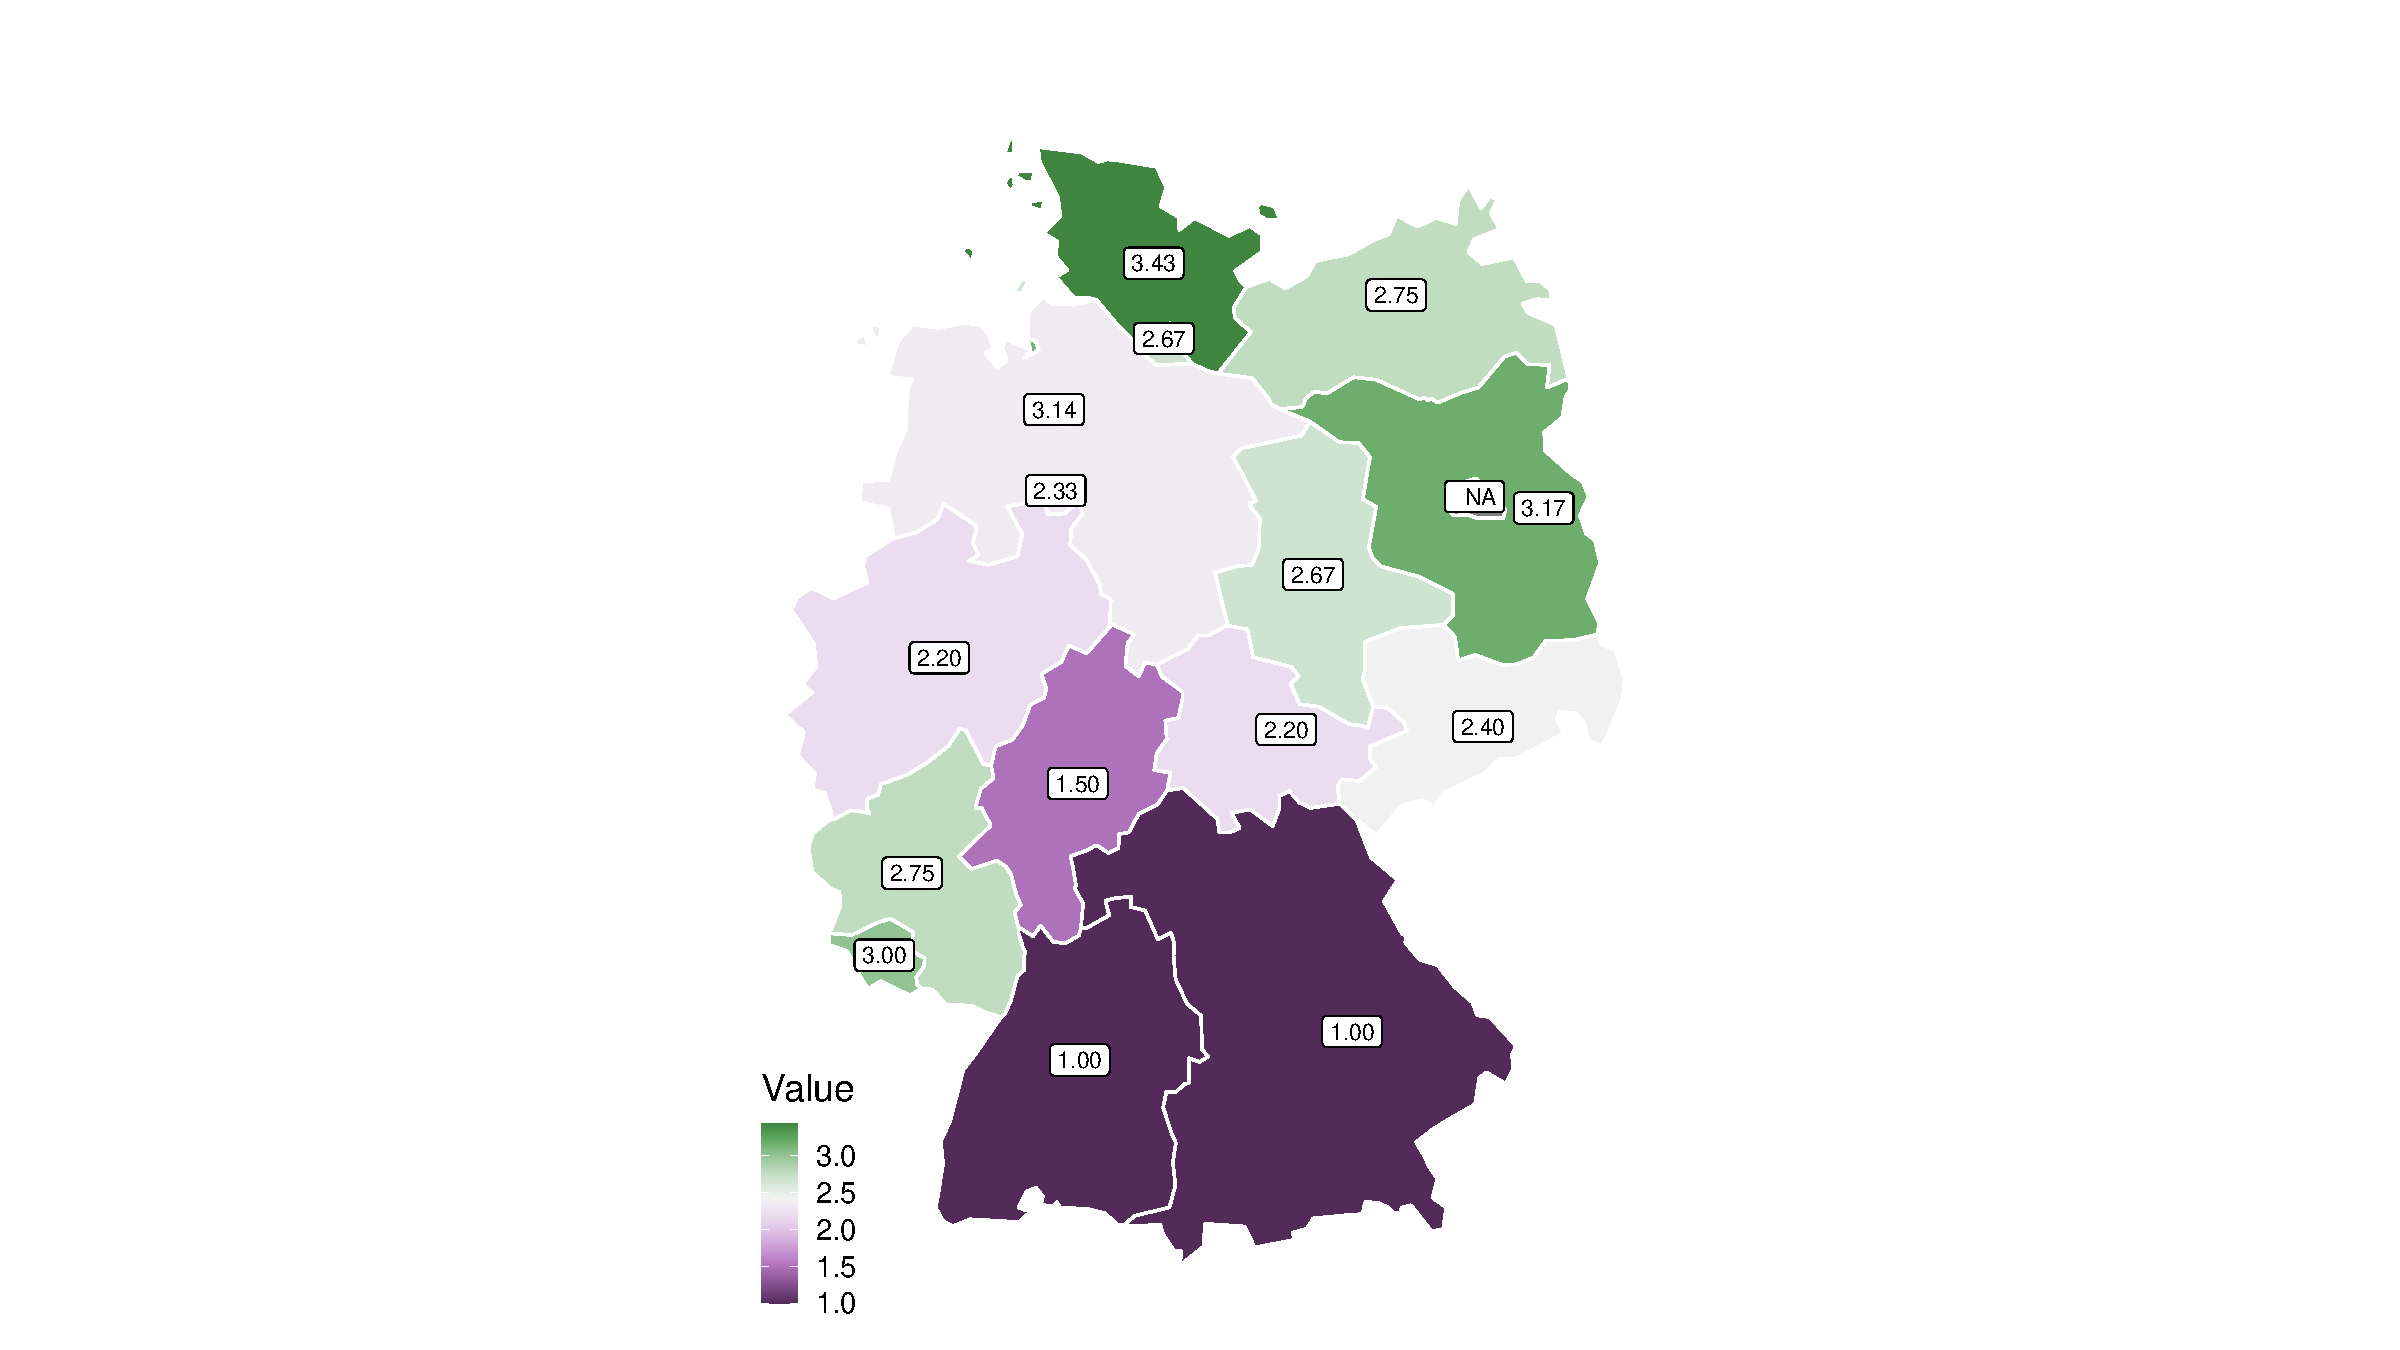
\includegraphics[width = \linewidth]{fedattAVG.pdf}
	\caption{States' attitudes toward federalism (average values). Source: \citep{BarbaroRode2024}}
%	\newline Attitudes toward federalism are measured on a scale of 1 (strongly federalistic, prefers decentralization) to 4 (strongly favors centralized decision-making)
    \label{fig.attitudemap}
\end{figure}


\end{document}
